\section{Model}
In this section the model of \projectname{} will be presented and explained using the UML notation described in Section~\ref{section:uml_notation}.
First the objects that need to be represented by the model are identified, and then their relationships are described. \\

The tables (and hence classes) have all been named according to the naming conventions in Rails \citep{ror_naming_convention}.

\subsection{Objects}
\label{subsec:objects}
The primary purpose of \projectname{} is to connect users and drones to allow the user to interact with a drone by watching its video feed, controlling its movements or both.
Therefore the users and drones are the primary objects that must be represented in \projectname{}. \\

The system will contain the following objects and relationships:

Objects:
\begin{itemize}
	\item User
	\item Company
	\item Role
	\item Privilege
	\item Drone
	\item Flightplan
\end{itemize}

The relationship between the objects can be seen in Figure~\ref{fig:UML_class_diagram}. 
This figure also serves as the model for the whole system. \\

\begin{figure}[htb]
    \centering
    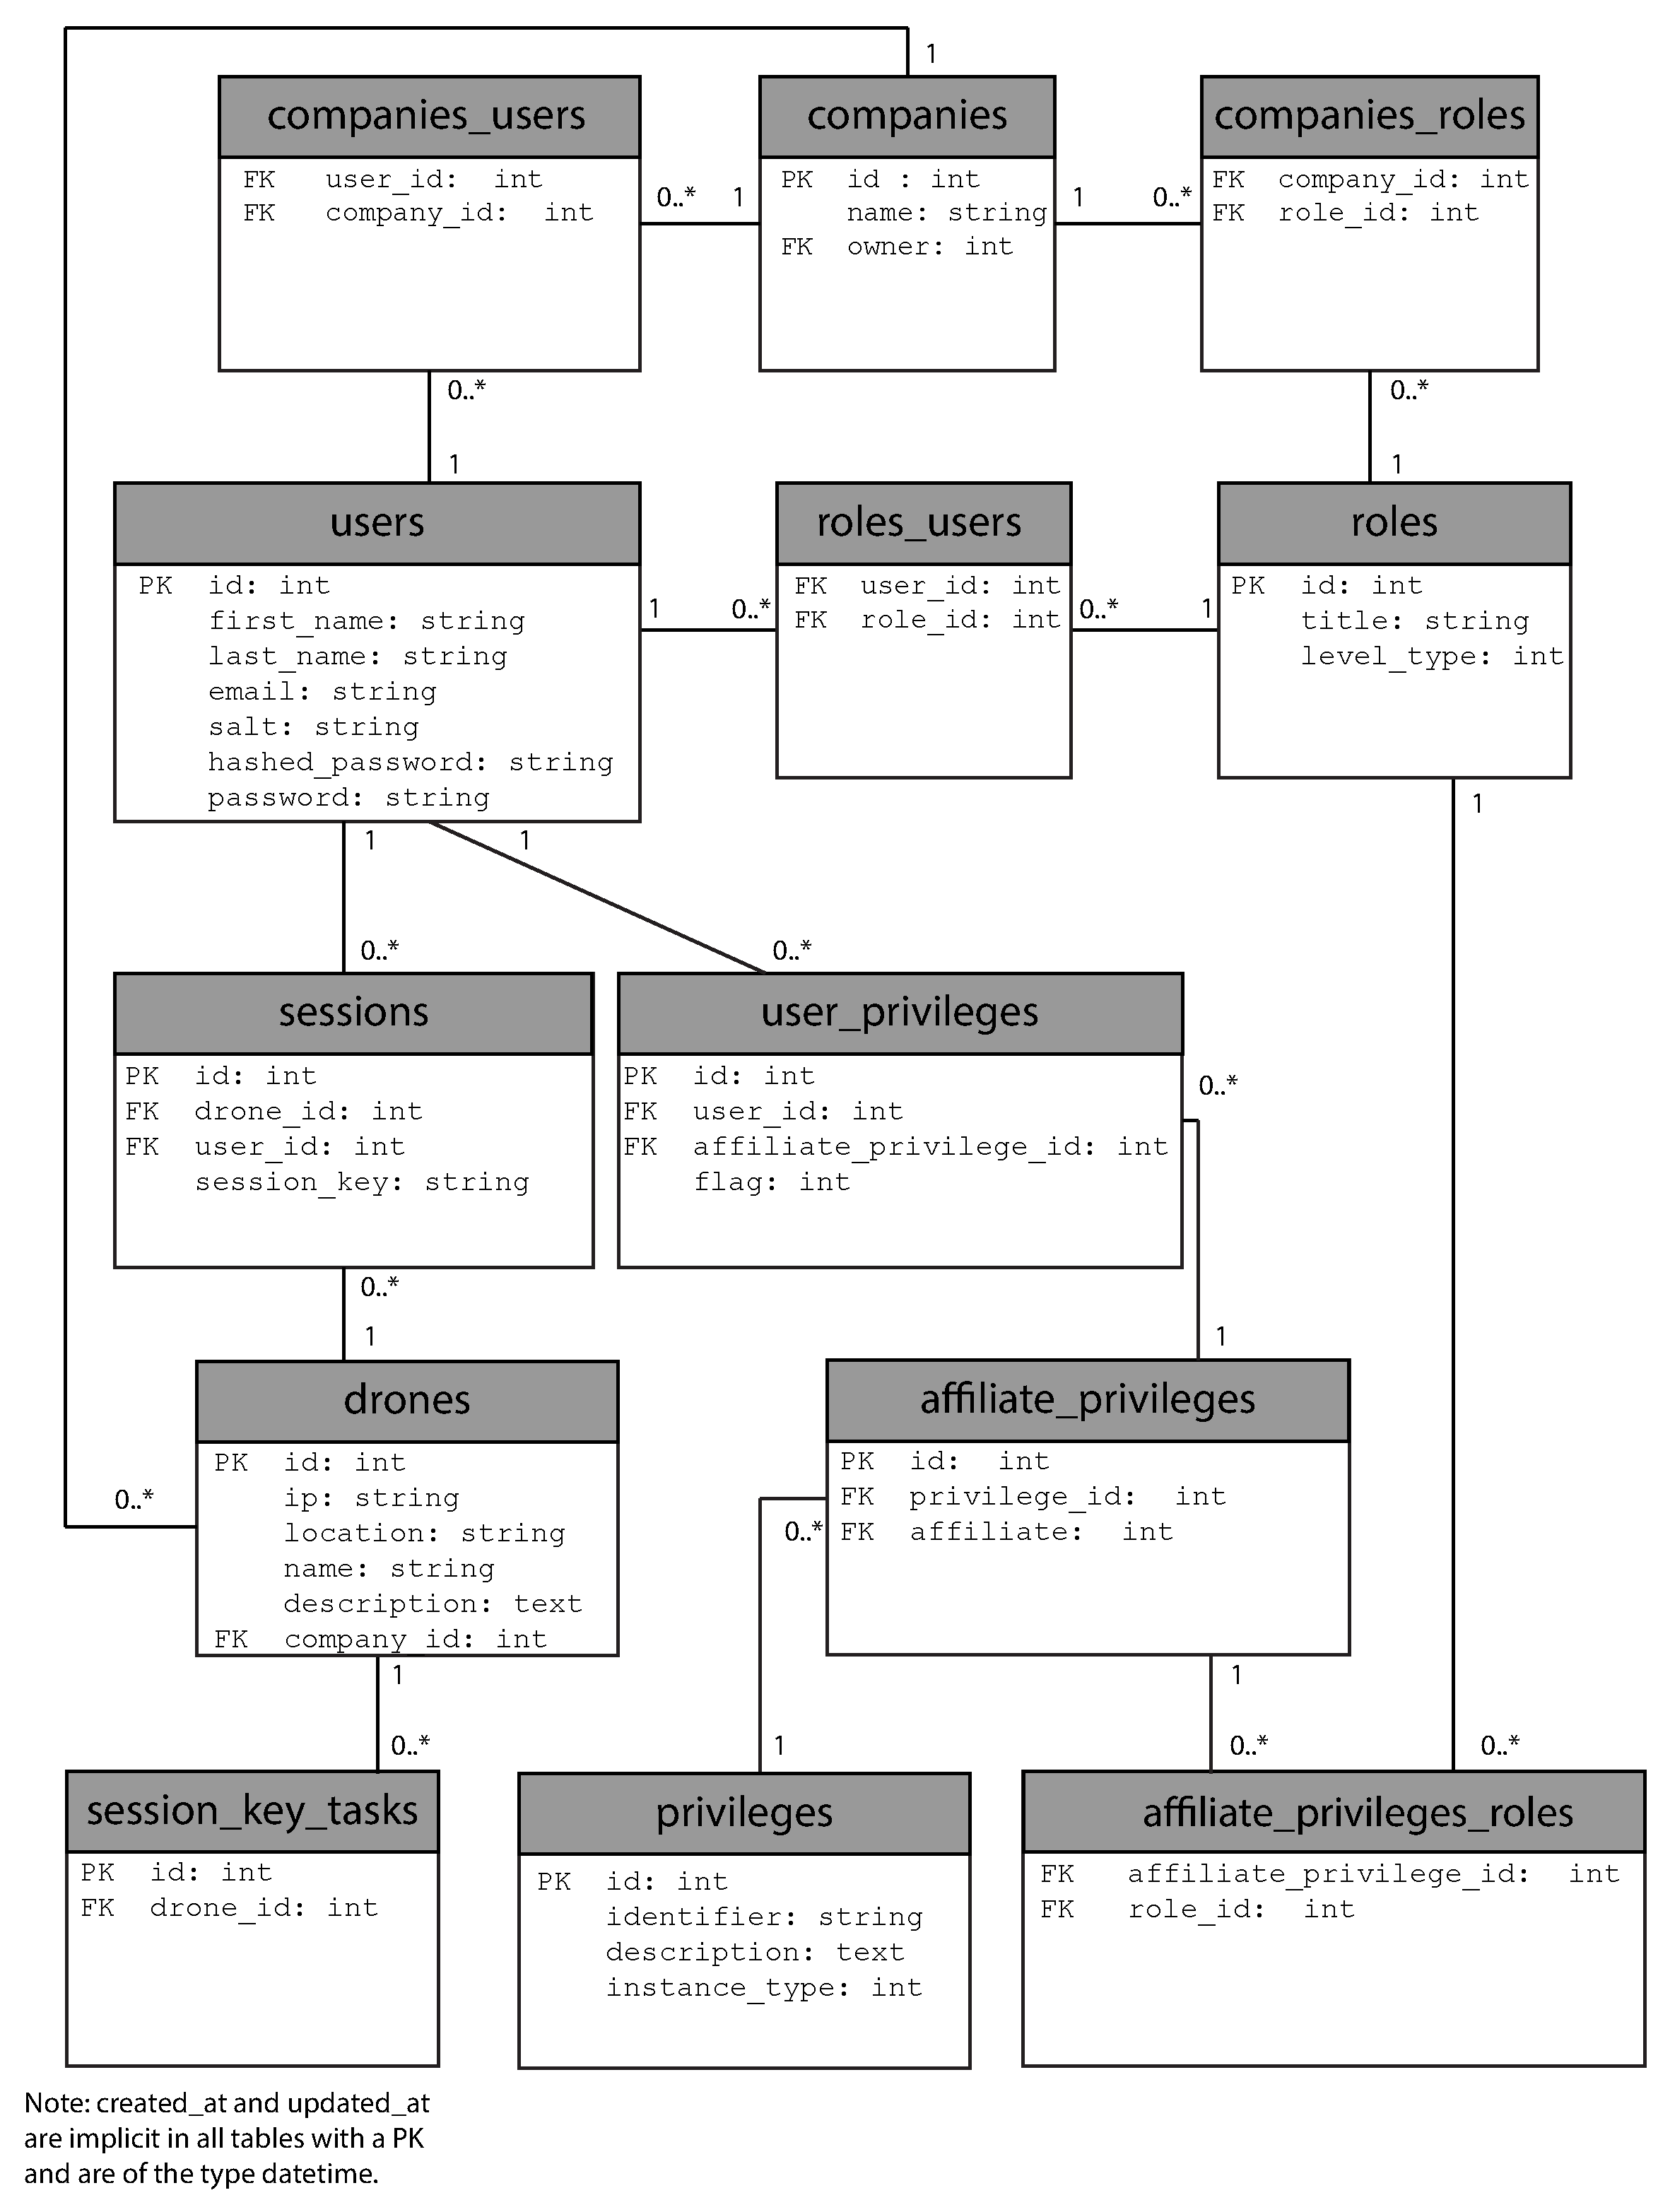
\includegraphics[width=\textwidth]{gfx/UML_model.pdf}
    \caption{UML Class Diagram of \projectname{}}
    \label{fig:UML_class_diagram}
\end{figure}

The follow section will analyse all the object types in the system, their relationships and why they are built as they are.
The upper part of Figure~\ref{fig:UML_class_diagram} shows the relationship between users, companies and roles/privileges while the lower part of the figure shows the relationship between drones, roles/privileges and flight plans. 


\subsubsection{User}
Only users that are logged in with a valid username and password can interact with the system.
If you are visiting the system as a guest and hence not logged in, only a login-page will be displayed. 
The system is designed so that every individual has their own unique user, allowing the system to show user-specific objects and allow user-specific access to different parts of the system. \\

A users access to the system will need to be restricted to make sure that any user only accesses what he is permitted too. 
This restriction is controlled by roles and privileges.
The handling of roles and privileges will be done by the role-model. \\

A user will be identified by his e-mail address which will work as the username and therefore be unique.
Each user will also have a password, that is both salted and encrypted in the database, using the SHA-1 encryption algorithm. \\

The user-object serves as the point of entrance for anyone who wishes to use the system, and combined with companies, roles and privileges dictate its options.


\subsubsection{Company}
\projectname{} is designed with the intent that multiple different clients can use the system.
These clients could be different companies that in some way wishes one or more drones to surveil their premisses.
One company may have several employees that they wish to provide with access to the system.
The Company-object handles this relationship, allowing multiple users to be grouped together by a company.
One User can be a member of several Company, and one Company can have many Users in it. 
Therefore this is a many-to-many relationship, represented in the Companies\_users table. \\

Roles and privileges can be assigned to a Company and inherited by its Users. 
This is described in further details in the following sections. 


\subsubsection{Drone}
Along with Users, Drones are the most important Object in \projectname{}.
An instance of a Drone in the system represents a physical drone somewhere in the field. 
A drone-object itself does not contain much data nor functionality. 
It simply represents a drone and is a point of connection between Users and controlling the Drone itself. \\

The relationship between a User and a Drone is controlled by Privileges and Drones through Companies in most cases. \\

The logging of when a drone takes of and lands is represented by the Flightplans table. 


\subsubsection{Flightplan}
Flightplans are used to log whenever a drone takes of and lands and which user is issuing the commands. 
One drone can have many flight plans.
One flight plan can have one drone. 
Therefore this is a one-to-many relationship. 


\subsubsection{Privilege}
\label{sec:privileges}
A privilege-object represents a privilege that can be granted to another object in the system. 
Examples of privileges are:

\begin{itemize}
	\item Add a new user to the system
	\item Edit the informations of a specific company
	\item Watch the video feed from a specific drone
	\item Control the movement of a specific drone
\end{itemize}

A privilege consists of three elements:

\begin{itemize}
	\item An action that it provides privilege to perform (such as any of the ones mentioned above)
	\item An object that these can be applied on
	\item An affiliation where the privilege is provided too. 
\end{itemize}

Privileges are not assigned to Users or Companies though, but referenced too by a Role.


\subsubsection{Role}
Roles are the glue that binds Users, Drones and Privileges. 
Consider a role as a collection of Privileges that are assigned to an object in the system.
Roles can be assigned to:

\begin{itemize}
	\item Users -- in this case, it is the same as if the privileges were granted directly to the user.
	\item Company -- in this case, the company administrator can assign users in the company to any of the assigned roles.
\end{itemize}

Roles are not the only way that a user can get a privilege granted, however. 
Though a user can be granted all privileges in a role by getting assigned to it, a user is also able to be granted a privilege directly via the \verb+User_Privileges+ table.


\subsection{Relationships}
The system is designed with flexibility and scalability in mind, and the structure of roles and privileges are what provides those features. 
As described before there are two ways a user can be granted a specific privilege. 
These are by 1) getting the privilege granted directly via the \verb+User_Privileges+ table or 2) by being a member of a Role that via the \verb+Privileges_Roles+ table that has one or more privileges granted. 
These will be explained in details in the following subsections. 


\subsubsection{Users and Privileges}
\label{sec:users_and_privileges}
An administrator can grant a specific privilege directly to a user via the \verb+User_Privileges+ table. 
This privilege is then affiliated with an object -- usually a Drone. 
The privilege could also be a system functionality, however, as described in Section~\ref{sec:privileges}. \\

This relationship is also used for exceptions.
In an example where 5 Users U1, U2, U3, U4 and U5 are a member of a Role R1, we may have a situation where U2 is not suppose to have access to a given privilege P1 in R1. 
Then a User-specific privilege is granted to U2 on P1, but with the ``exception''-flag marked.
This is equal to blacklisting U2 from using privilege P1, providing the system with a lot of flexibility, as even though a group of Users are granted a number of privileges via a role, User-specific exceptions can be added to this setting. \\


\subsubsection{Roles and Privileges}
As mentioned before -- the reason that Roles can be used to assign Privileges to a User, is to make both the administration and data structure of users and privileges as simple and efficient as possible. 
By allowing exceptions, full flexibility is still possible. \\

This is how the relationship between Roles and Privileges works: \\

An administrator creates a Role.
Lets call this Role ``Control Drone \#4''.
A number of privileges are assigned to this Role.
It could be the following:

\begin{itemize}
	\item Watch the video feed from a specific drone
	\item Control the movement of a specific drone
\end{itemize}

Those privileges are then linked to this Role and to the drone this concerns. \\

Roles can be assigned with affiliation to both Users and Companies.
Say a user \verb+U1+ needs access to Drone \#4. 
User U1 then needs to either have the privilege directly granted as described in Section~\ref{sec:users_and_privileges} or be a member of the role ``Control Drone \#4''.


\subsubsection{Privileges and Drones}












\begin{comment}

A users' access to the system will need to be restricted to make sure that any user only access what he is permitted to.
This restriction will be represented through privileges that grant a user access to different system functionalities.
However, granting privileges directly to a user is not the ideal case in most situations, as a lot of duplicate data can occur.
The system will contain global privileges all users need access to.
Assigning global privileges to each user individually is not an ideal solution.
Therefore this will be handled via roles.
A role will in \projectname{} be a set of privileges and assignable to multiple users.
When assigning a user to a role, the user will automatically get access to any privilege granted to that role.
By doing it that way, a lot of privilege gratings can be saved by adding all users that needs the same privileges to a role. \\

%A drone is controlled by sending a set of ordered instructions\fixme{ref to section when it is written} to the drone.
%A log of flights made by the drone will need to be kept, to be able to recreate previous flights, and examine a flight that might have caused the drone to crash.
%This log will be referenced in the system as a flight plan.
%A flight plan will consist of a set of actions taken by the drone, each referencing a specific instruction send to the drone.

A structured list of the objects can be seen in Figure~\ref{tab:model_objects}.

\begin{figure}[H]
\begin{center}
\begin{tabular}{ |c| }
  \hline
	\textbf{Object}\\ \hline
	User \\ \hline
	Role \\ \hline
	Privilege \\ \hline
	Drone \\ \hline
	%Flight plan \\ \hline
	%Action \\ \hline
	%Instruction\\ \hline  
\end{tabular}
\caption{The objects that will be present in the system.}
\label{tab:model_objects}
\end{center}
\end{figure}

\subsection{Model Diagram}
A diagram of the model can be seen in Figure~\ref{fig:UML_class_diagram}.
It should be noted all tables are named according to the naming conventions in ROR\citep{ror_naming_convention}.
The upper part of Figure~\ref{fig:UML_class_diagram} shows the relationship between users, roles, companies, and privileges.
In the following section all references to tables refer to the tables seen in Figure~\ref{fig:UML_class_diagram}

\subsubsection{User Privilege Relationship}
As mentioned in Section~\ref{subsec:objects} a role in \projectname{} is a set of privileges.
A role is linked to a set of privileges through the relationship table \verb+Privilege_roles+.
In Rails this relationship is referred to as a many to many association, as a user can be associated with many roles and a role can be associated with many users.
\verb+Privilege_roles+ links the ids of roles to the ids of privileges.
Users and roles are linked in the same manner as roles and privileges.
In the table \verb+Role_Users+ the ids of users to the ids of roles are linked.

\begin{figure}[htb]
    \centering
    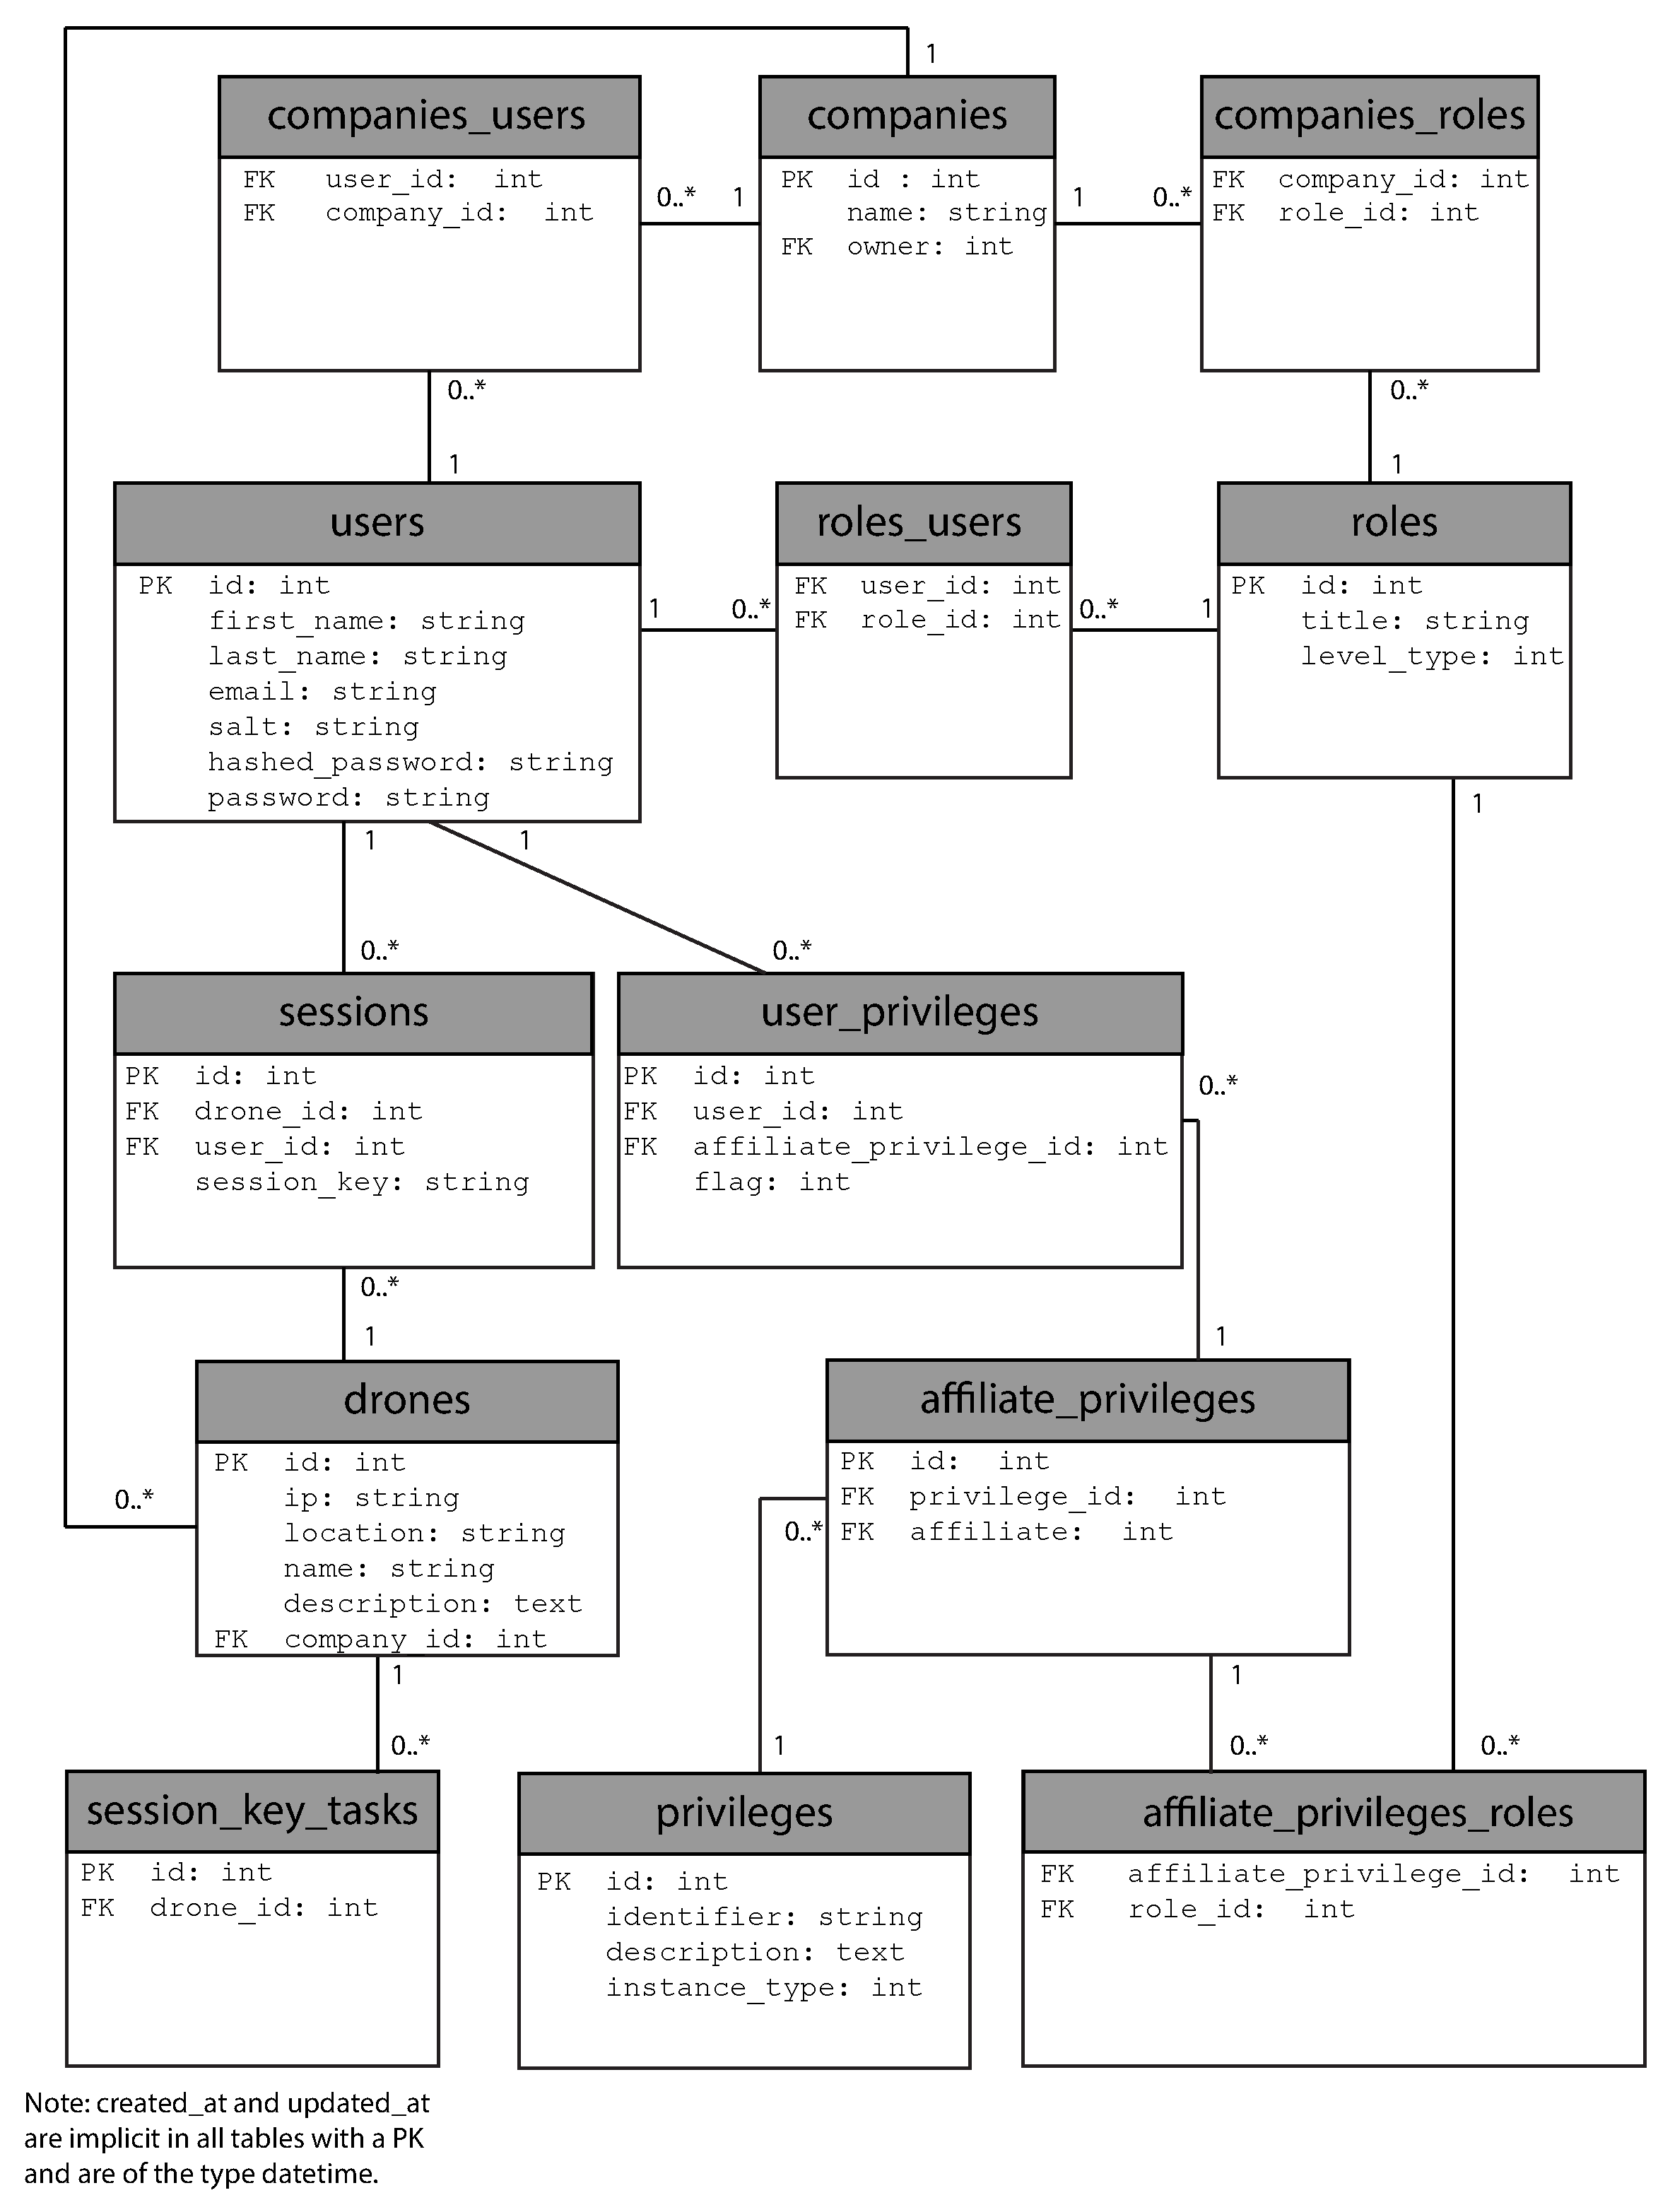
\includegraphics[width=\textwidth]{gfx/UML_model.pdf}
    \caption{UML Class Diagram of \projectname{}}
    \label{fig:UML_class_diagram}
\end{figure}

However, linking privileges to users only through roles creates cases were maintaining privileges can become troublesome.
As an example a user \verb+u+ might need to have his access to a specific privilege \verb+p+ in a role \verb+r+ that he is a member of, revoked.
A possible solution is to remove the user from \verb+r+ and add him a to new role \verb+r1+ that contains all privileges in \verb+r+ except \verb+p+.
The problem with this solution arises if a new privilege \verb+p1+ is to be added to \verb+r+.
The user \verb+u+ is implicitly a member of \verb+r+, but has the role \verb+r1+ to exclude him from the privilege \verb+p+.
To grant \verb+p1+ to \verb+u+, \verb+p1+ must be added to \verb+r1+ as well as \verb+r+.
Granting privileges only through roles can therefore quickly result in a lot of unstructured data that needs to be maintained. \\

To handle this, users are linked directly to privileges through the relationship table \verb+User_Privileges+.
This table differs from the other relationship tables as it does not just link to id foreign keys.
In Rails, this is referred to as a rich many-to-many associated.
In a rich many-to-many association additional, fields are added to the relationship table.
In \verb+User_Privileges+ users and privileges are linked through ids, with an extra field containing a flag.
This flag defines if the privilege the user is linked to is whitelisted or blacklisted through the relation.
This design makes management of privileges more flexible.

Groups of privileges can be assigned through roles, and should a case arise where a users privileges need to be managed individually this is possible through the \verb+User_Privileges+ relation.

\subsubsection{User Companies Relationship}
Users can grouped together via an entity -- this system define as a Company.
A user can via Companies\_users be linked to a company with the foreign keys of both the user and the company. 
A company can via the Company\_roles table be linked to a role in the same way that a user can be, using the foreign keys for the company and the role. 
This will grant the privileges in the role to all users associated with this company.
Finally a drone can be connected to a company via the Company\_drones table, that also uses foreign keys. 
This is to define which drones are associated with a company.
In the case where a company administrator needs to edit the privileges for a drone in accessible for the company, he needs to be able to see which drones are actually associated with the company. 
That list is made via this many-to-many reference. 

\subsection{Drone Flight Plan Relationship}
The flight logging system consists directly of the classes \verb+Drones+, \verb+Flight_plan+ and \verb+Actions+.
Drones are linked to flight plans through a foreign key.
A flight plan is connected to a set of actions through a one-to-many relation.
The actions must be numbered representing the order in which the actions were send to the drone.
This numbering will be managed in the \verb+Flight_Action_Relationship+ with the field \verb+rank+.
An action will be linked to an instruction.
Instruction represent the set of AT commands that can be send to the drone to control.\fixme{Ref til AT command sektion n�r den skrives}

Through this model the log for a flight with a given drone can be extracted by locating all action associated with the flight plan through the \verb+Flight_Action_Relationship+.

\end{comment}



%\subsection{Privileges}
%A user is granted privileges through a whitelist.
%Every privilege not found in a users whitelist is implicitly blacklisted.
%As described in Section~\ref{subsec:objects} a user can be granted privileges through roles.
%There are however a set of cases where handling privileges only through roles is not ideal.
%As an example a user \verb+u+ might need to have his access to a specific privilege \verb+p+ in a role \verb+r+, he is a member of, revoked.
%A possible solution is to remove the user from \verb+r+ and add him a to new role \verb+r1+ that contains all privileges in \verb+r+ except \verb+p+.
%The problem with this solution arises if a new privilege \verb+p1+ is to be added to \verb+r+.
%The user \verb+u+ is natively a member of \verb+r+, but has the role \verb+r1+ to exclude him from the privilege \verb+p+.
%To grant \verb+u+ \verb+p1+, \verb+p1+ must be added to \verb+r1+ as well as \verb+r+.
%Granting privileges only through roles can therefore quickly result in a lot of unstructured data that needs to be maintained.
%To solve privileges need to be manageable on the user level.


%As an example a user might need a specific privilege that allows him to fly a specific drone.
%Adding the user to a group \verb+p+ with that privilege would not work as he would then additionally receive every other privilege in \verb+p+.
%The problem can be solved by giving each user a personal role containing all their uniquely assigned privileges.